\documentclass[10pt,a4paper,twocolumn]{article}

\usepackage{cvpr}
\usepackage{times}
%\usepackage{epsfig}
\usepackage{graphics}
\usepackage{graphicx}
\usepackage{amsmath}
\usepackage{amssymb}
\usepackage{wrapfig}
\usepackage{subcaption}
\usepackage[breaklinks=true,bookmarks=false]{hyperref}
\usepackage{float}
\cvprfinalcopy

\begin{document}

%%%%%%%%% TITLE
\title{\textsf{Advanced Algorithms project report}}

\author{Giacomo Fabris\\
University of Trento\\
{\tt\small giacomo.fabris-1@studenti.unitn.it}
}

\maketitle
%\thispagestyle{empty}

\section{Introduction}

%-------------------------------------------------------------------------
Objective of the project is to create a classifier which is able to determine which illness (if any) affects the lungs of a patient, based on their thoracic X-rays images. Illnesses shall be classified in 4 categories: none, bacterial infection, COVID-19, viral infection (non-COVID).

The dataset on which the classifier is trained is composed of about 6000 examples, made of (a) the black-white thoracic X-rays image, 256 pixel wide and high, and (b) a feature vector of 84 entries, extracted from the image. Of the entire dataset, ~60\% shall be considered for training, ~20\% for validation and ~20\% for testing. It shall be noted that the amount of examples for each class varies greatly: the examples of COVID-19 are very few compared to the other classes, which are more equally represented.

Performance shall be measured as the average over classes of the sensitivity, i.e. the proportion of examples from a given class correctly identified as such. 

\section{Proposed Method}

I considered the use of neural networks to solve the classification task, performing two main experiments:
\begin{enumerate}
    \item using as input the feature vectors only, I implemented a simple fully connected feed-forward neural network;
    \item using as input both the pictures and the feature vectors, I implemented a (small) deep neural network, composed of a convolution stage on the image and a fully-connected stage which collects the output of the CNN and the feature vector, producing the output.
\end{enumerate}

\subsection{Fully connected network on feature vectors}

The feed-forward neural network is composed of 4 layers of, respectively, 84, 42, 21 and 4 perceptron.
Increasing further the number of layers had no sensible effect on the precision of the model; similarly, the effect of changing the number of perceptrons of each hidden layer was not dramatic, above a certain threshold.

I experimented with two optimizers, Stochastic Gradient Descent and Adagrad, and with two activation functions, ReLU and sigmoid. The final evaluation has been performed with the Adagrad optimizer, setting an initial learning rate of 5e-4, without weight decay. ReLU has been chosen as activation function. The training has been scheduled using a multi-step learning rate scheduler with a milestone at the 20th epoch; the entire learning lasts 35 epochs. The loss function being used is a weighted cross-entropy loss, where weights compensate the fact that the dataset is not homogeneous in terms of number of instances. For any class $C$ of the dataset $D$, the weight has been set to $1000{|C|}^{-1}$; alternative weights of ${|C|}^{-2}$ and $|C|^{-0.5}$ has been considered but resulted in an unbalanced true positive rate between classes.

\subsection{Deep network on image dataset}

The deep network is composed of two main segments. The first involves the image processing, and is composed of two main convolution steps, while the second is a feed-forward network which processes the output of the convolution network and the feature vector input. ReLU is chosen as activation function for each step of the network.

Each convolution step is composed of a convolution layer with kernel size 5*5 and stride 1; a dropout layer with $p = 0.2$ is inserted after each convolution; then, max pooling with a 3*3 filters is performed to reduce dimensionality.

The output tensor is then linearized and fed into a first layer of perceptrons and normalized, the same processing is performed on the feature vector. Then, the results of the two normalizations are concatenated together into a single vector, which goes through an additional dropout layer with $p = 0.2$ and two perceptron layers.  

The network comprises dropout layers because while experimenting I had issues with overfitting, thus I considered both L2 regolarizers (weight decay) of the loss function and dropout layers; I chose the latter because it yielded a better performance of the model in terms of the accuracy measure defined in the problem statement.

Training has been performed using the Adagrad optimizer, setting an initial learning rate of 1e-3. Similarly to the previous network, the loss function is cross-entropy loss, whose weights have been set proportional to the inverse of the number of examples of each class.

\begin{figure}[H]
    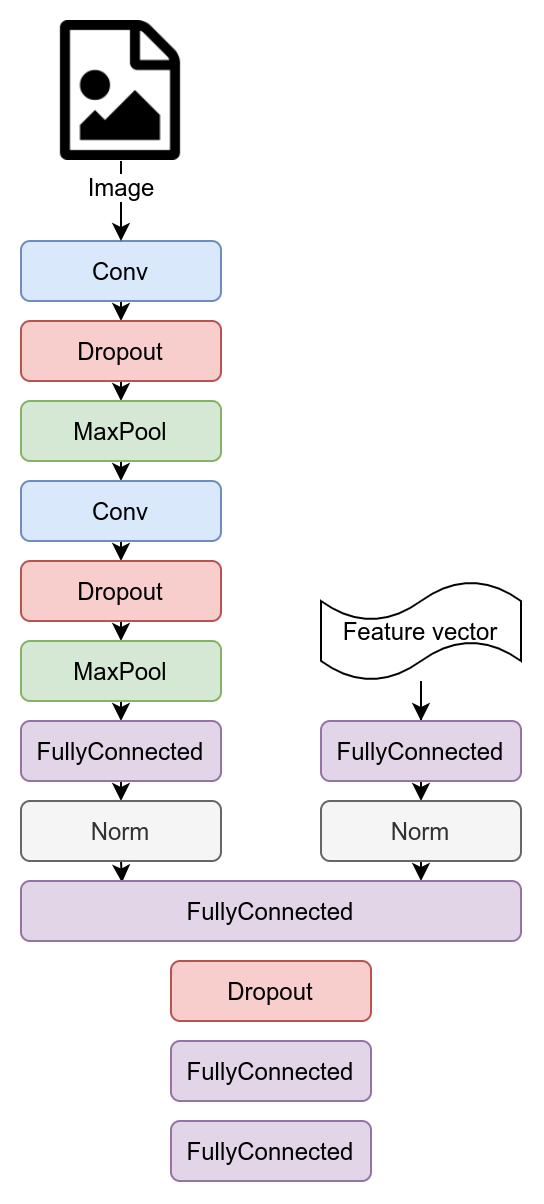
\includegraphics[width=0.7\linewidth]{Network.png}
    \caption{Deep network structure}
\end{figure}


\section{Results}

The algorithm has been implemented using PyTorch; the original source code is contained in the \texttt{src} directory of the attached archive.
The folder \texttt{models\_saved} contain the trained network and the run log of the experiments reported in this section. The \texttt{models} subfolder contains the serialized weights of the network, which may be loaded by the \texttt{nn.py} or \texttt{deepnn.py} source file; the \texttt{output} subfolder contains the test run output and the \texttt{tb\_logs} subfolders contain the telemetry data of the training collected using tensorboard.
The folder \texttt{report} contains the source file of this document and the code used for the generation of plots.

The following graphs show two experiments, one with each network described in the previous section; the performance after each epoch is evaluated and the final confusion matrix is shown.

\begin{figure}
    \centering 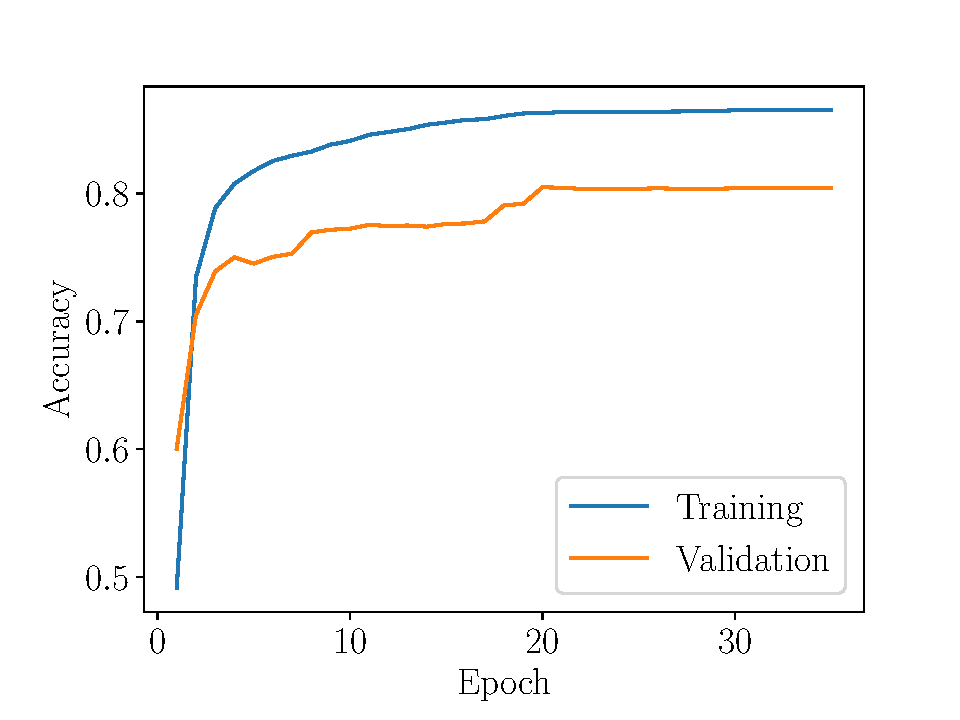
\includegraphics[width=\linewidth]{plot_nn_macc}
    \caption{Network \#1: learning performance}
\end{figure}

\begin{figure}
    \centering 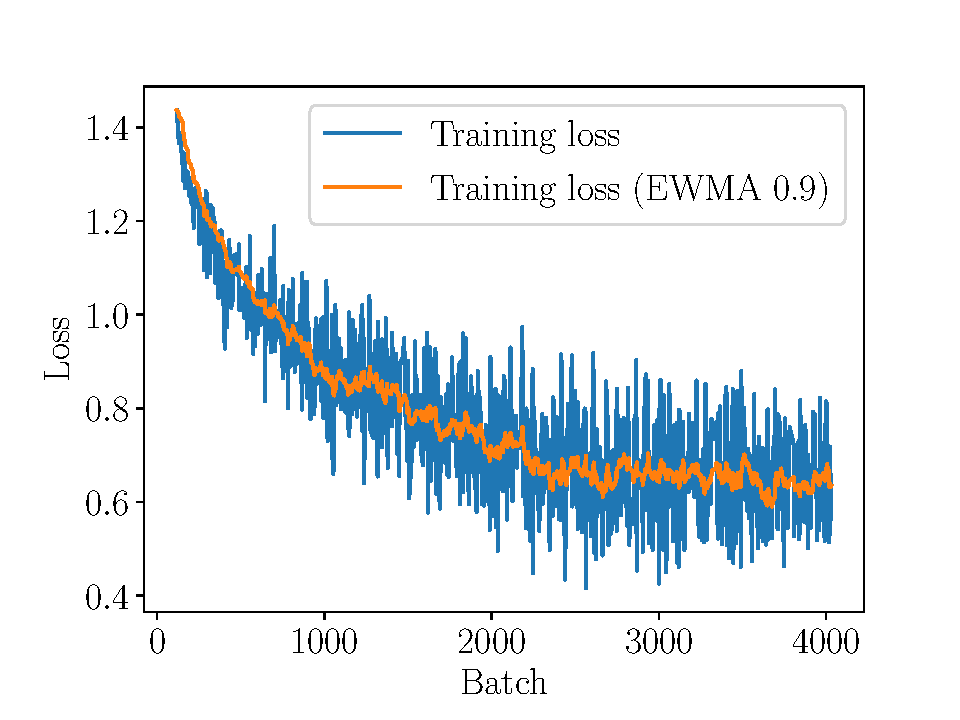
\includegraphics[width=\linewidth]{plot_nn_loss}
    \caption{Network \#1: loss value of each training batch}
\end{figure}

\begin{figure}
    \centering 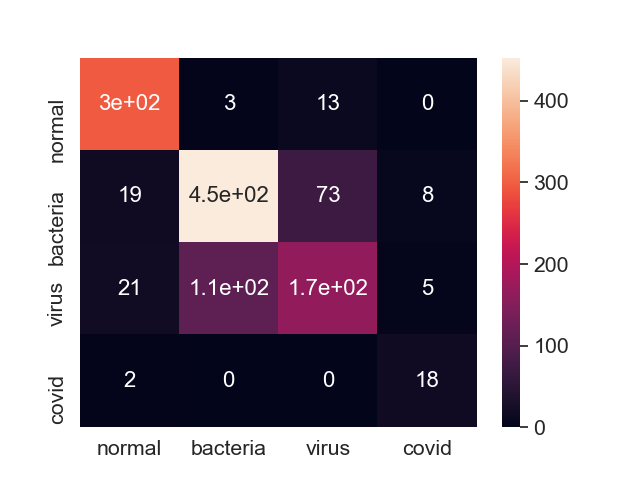
\includegraphics[width=\linewidth]{nn_confusion}
    \caption{Network \#1: confusion matrix}
\end{figure}

\begin{figure}
    \centering 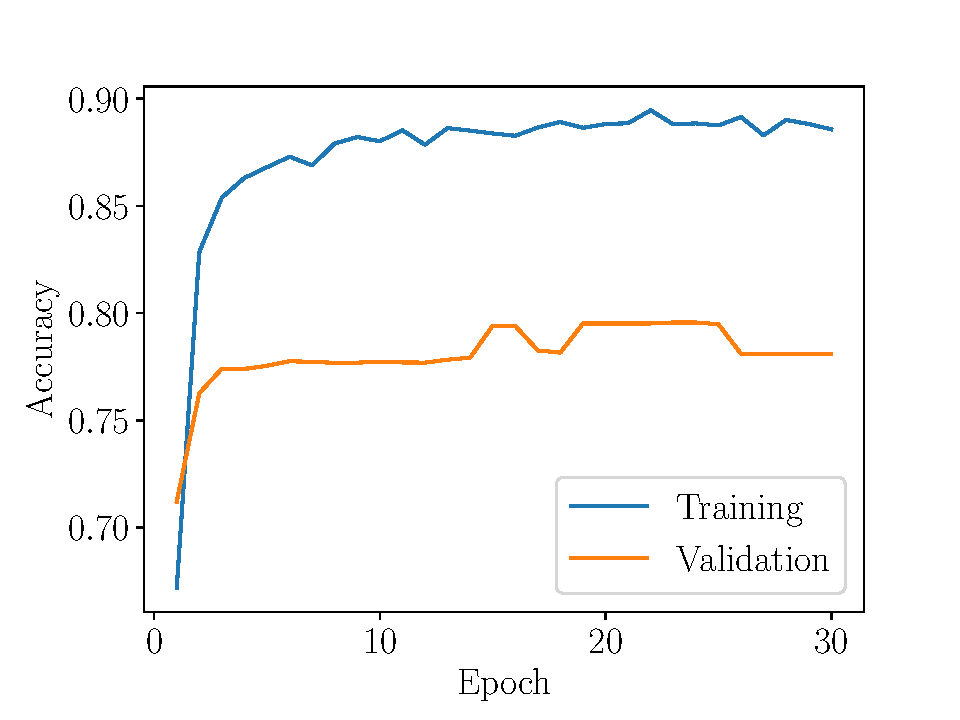
\includegraphics[width=\linewidth]{plot_dnn_macc}
    \caption{Network \#2: learning performance}
\end{figure}

\begin{figure}
    \centering 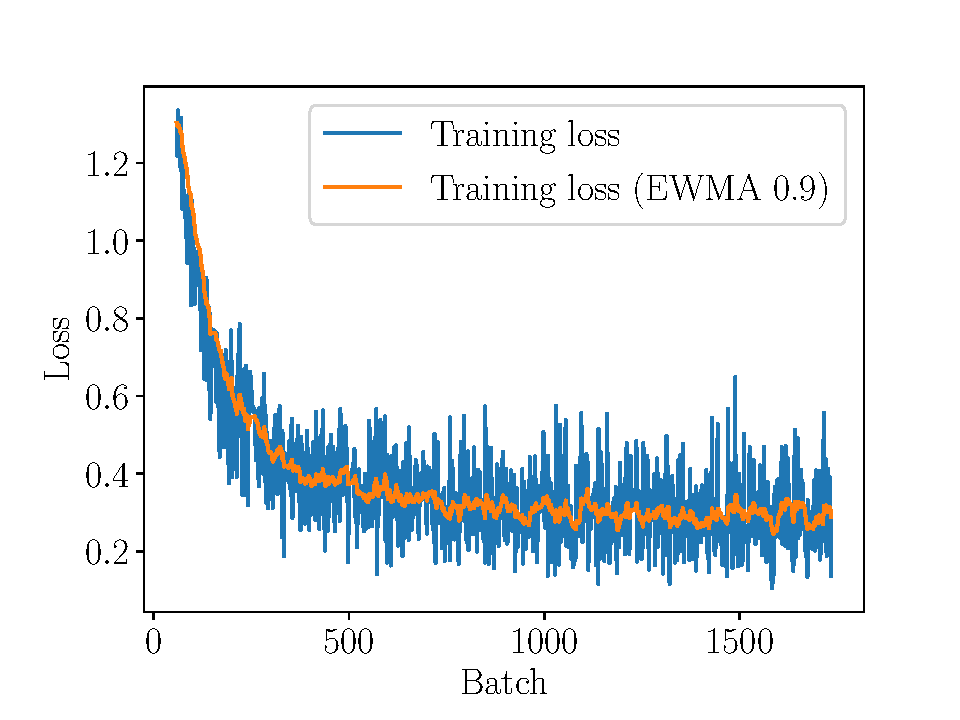
\includegraphics[width=\linewidth]{plot_dnn_loss}
    \caption{Network \#2: loss value of each training batch}
\end{figure}

\begin{figure}
    \centering 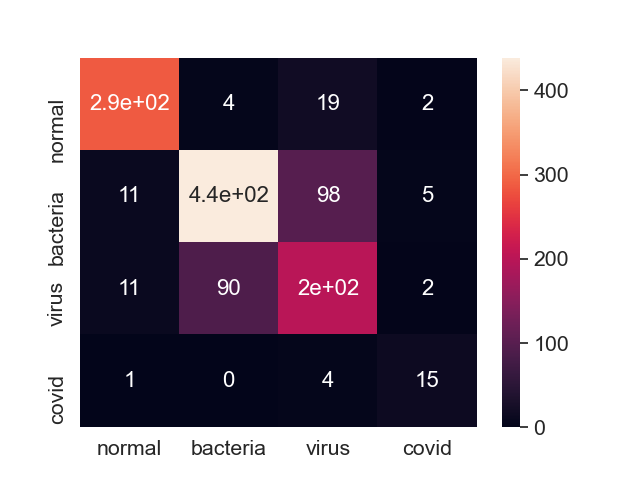
\includegraphics[width=\linewidth]{dnn_confusion}
    \caption{Network \#2: confusion matrix}
\end{figure}


%{\small
%\bibliographystyle{ieee}
%\bibliography{egbib}
%}

\end{document}
